
\subsection{Sensorik}


\subsubsection{Gyroskop}
Funktionsweise
Tiefpassfilter
Bias-Korrektur
HBW \& LBW Fusion
Wertebereiche, wie alte Präsentation
Integration
Eigenschaften (schnell, aber Drift durch Integration)


\subsubsection{Beschleunigungssensor}
Funktionsweise
für Roll und Pitch
Tiefpassfilter
Umrechnung auf m/s$^2$
Berechnung von Roll und Pitch direkt aus Werten
Problem: ungenügendes Yaw


\subsubsection{Magnetometer}
Das Magnetometer wurde im Rahmen des Praktikums zur Stützung des Yaw-Winkels (Drehung um die Z-Achse im Brillenkoordinationsystem) genutzt.\\
Das verbaute Magnetometer misst in drei Achsen nach dem Funktionsprinzip der Wheatstonesche Messbrücke \cite{renaudin2010complete} das Erdmagnetfeld. Dieses Messverfahren führt zum einen zu einer kleinen und kostengünstigen Bauweise. Zum anderen entstehen durch dieses Funktionsprinzip Messungenauigkeiten, die im Rahmen der Sensorkalibrierung beachtet und ausgeglichen werden müssen.\\
Der gemessene 3D-Magnetfeldvektor ist somit zunächst unkalibriert und laut der Spezifikation im Datenblatt \todo{cite} einheitenlos.
Daher war zuerst eine Kalibrierung der gemessenen Werte notwendig um sie weiterverarbeiten zu können. Im Gegensatz zu den bisher vorgestellten Sensoren wird die Kalibrierung des Magnetometers durch Bewegung durchgeführt. Ziel ist es die Wertebereich in allen drei Achsen zu erfassen. Dafür wird die Brille in allen Achsen um mindestens $360^\circ$ gedreht um die minimalen und maximalen Werte zu registrieren. \ldots Wie in Abbildung \ref{fig:mag_world}\ldots



Funktionsweise

\begin{figure}
   \centering
   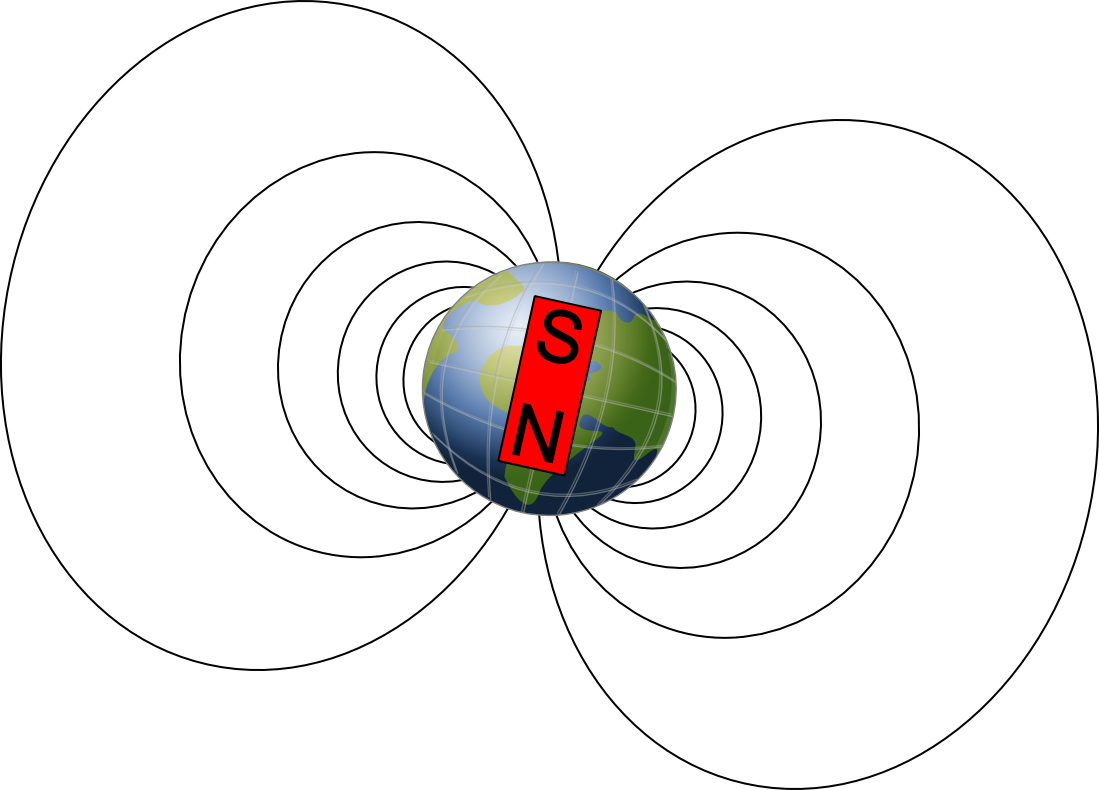
\includegraphics[width=0.3\textwidth]{earth-magnetic-field}
   \caption[mag_world]{Schematische Darstellung des Erdmagnetfelds.}
   \label{fig:mag_world}
\end{figure}


Tiefpassfilter
Magnetometer-Bias-Korrektur (durch Min/Max-Werte), Normierung auf [-1,1]
Magnetometer-Kreisplots vor/nach Kalibrierung, Magnetometer-Fehler in Kreisplots
Transformation auf XY Ebene (Algorithmus Ralf)


\subsubsection{Kamera}

